\documentclass[reqno, 12pt]{amsart}
\usepackage{enumerate}
\usepackage{amsmath}
\usepackage{scrextend}
\usepackage{bm}
\usepackage{algorithm}
\usepackage{algpseudocode}
\usepackage{graphicx}
\usepackage{enumitem}
\usepackage{tcolorbox}
\usepackage[headheight=12pt,textwidth=7in,top=1in, bottom=1in]{geometry}
\usepackage{listings}
\usepackage{cancel}
\usepackage{color} %red, green, blue, yellow, cyan, magenta, black, white
\definecolor{mygreen}{RGB}{28,172,0} % color values Red, Green, Blue
\definecolor{mylilas}{RGB}{170,55,241}
\usepackage{dirtree}

\usepackage[]{xcolor}
\definecolor{lightblue}{rgb}{0.63, 0.74, 0.78}
\definecolor{seagreen}{rgb}{0.18, 0.42, 0.41}
\definecolor{orange}{rgb}{0.85, 0.55, 0.13}
\definecolor{silver}{rgb}{0.69, 0.67, 0.66}
\definecolor{rust}{rgb}{0.72, 0.26, 0.06}
\definecolor{purp}{RGB}{68, 14, 156}

\colorlet{lightrust}{rust!50!white}
\colorlet{lightorange}{orange!25!white}
\colorlet{lightlightblue}{lightblue}
\colorlet{lightsilver}{silver!30!white}
\colorlet{darkorange}{orange!75!black}
\colorlet{darksilver}{silver!65!black}
\colorlet{darklightblue}{lightblue!65!black}
\colorlet{darkrust}{rust!85!black}
\colorlet{darkseagreen}{seagreen!85!black}

\usepackage{hyperref}
\hypersetup{
  colorlinks=true,
}

\hypersetup{
  linkcolor=darkrust,
  citecolor=seagreen,
  urlcolor=darkrust,
  pdfauthor=author,
}

\usepackage{cleveref}

%some custom commands you may find useful
\usepackage{xparse}
\DeclareDocumentCommand{\diff}{O{} m}{
	\frac{\mathrm{d} #1}{\mathrm{d}#2}
}
\DeclareDocumentCommand{\difftwo}{O{} m}{
	\frac{\mathrm{d}^2 #1}{\mathrm{d}#2^2}
}
\DeclareDocumentCommand{\pdiff}{O{} m}{
	\frac{\partial #1}{\partial #2}
}
\DeclareDocumentCommand{\pdifftwo}{O{} m}{
	\frac{\partial^{2} #1}{\partial #2^{2}}
}
\DeclareDocumentCommand{\integral}{O{} O{} m O{x}}{
	\int_{#1}^{#2} #3\ \mathrm{d}#4
}
\DeclareDocumentCommand{\sp}{}{
	\qquad \qquad \qquad }{
}
\NewDocumentEnvironment{solution}{}{
	\begin{addmargin}[2em]{0pt}
	}{\end{addmargin} \vskip0.25cm
}

\newenvironment{sysmatrix}[1]
{\left(\begin{array}{@{}#1@{}}}
	{\end{array}\right)}
\newcommand{\ro}[1]{%
	\xrightarrow{\mathmakebox[\rowidth]{#1}}%
}
\newlength{\rowidth}% row operation width
\AtBeginDocument{\setlength{\rowidth}{3em}}

\def\name{Ben Wilfong} %your name goes here
\def\ID{bwilfong3} %your cm goes here

%these packages create the footer and page numbering
\usepackage{fancyhdr}
\usepackage{lastpage}
\pagestyle{fancy}
\lhead{\name}
%%%%%%%%%%%%%%%%%%%%%%%%%%%%%%%%
\chead{ME 7751 Homework \#2}
%%%%%%%%%%%%%%%%%%%%%%%%%%%%%%%%
\rhead{Username: \ID}
\fancyfoot[C]{\footnotesize Page \thepage\ of \pageref{LastPage}}
\fancypagestyle{firststyle}
{ \renewcommand{\headrulewidth}{0pt}%
	\fancyhf{}%
	\fancyfoot[C]{\footnotesize Page \thepage\ of \pageref{LastPage}}
}

\lstset{frame=tb,
  language=[90]Fortran,
  aboveskip=3mm,
  belowskip=3mm,
  showstringspaces=false,
  columns=flexible,
  basicstyle={\footnotesize\ttfamily},
  numbers=none,
  numberstyle=\tiny\color{gray},
  keywordstyle=\color{darklightblue},
  commentstyle=\color{seagreen},
  stringstyle=\color{darkrust},
  breaklines=true,
  breakatwhitespace=true,
  tabsize=3,
}

\begin{document}
	\noindent
	\thispagestyle{firststyle}
	%\begin{tabular}{l}
		%{\LARGE \textbf{ME 7751: Intro to CFD} }\\
		%%%%%%%%%%%%%%%%%%%%%%%%%%
		%{\Large Homework Set \#2}
		%%%%%%%%%%%%%%%%%%%%%%%%%%
	%\end{tabular} \hfill \begin{tabular}{r}
		%\name \\
		%Username: \ID
	%\end{tabular}
	%\noindent\makebox[\linewidth]{\rule{\textwidth}{1pt}}

    \begin{center}
        \LARGE{\textbf{Solution of the 2D steady heat equation with the finite difference method}} \\
        \Large{September 30$^{th}$, 2024} \\
        \large{Ben Wilfong}
    \end{center}
    \section*{Files}
    \dirtree{%
         .1 HW2\_root.
         .2 CMakeLists.txt.
         .2 homework.pdf.
         .2 main.inp.
         .2 make.sh.
         .2 src.
         .3 m\_global\_parameters.f90.
         .3 m\_helpers.f90.
         .3 m\_iterative\_methods.f90.
         .3 p\_main.f90.
         .2 plots.
         .3 *.csv.
         .3 plots.m.
    }
    \section*{Compiling}
    \noindent This code can be compiled in a terminal by running \texttt{chmod u+x ./make.sh} followed by \texttt{./make.sh} in the \texttt{HW2\_root/} directory.
    This will compile and link the source code in the \texttt{src/} directory and create an executable called \texttt{main} in the \texttt{HW2\_root/} directory.
    \section*{Running}
    \noindent The problem parameters are defined in the namelist file \texttt{main.inp} in \texttt{HW2\_root/}.
    The input parameters are:
    \begin{itemize}
        \setlength\itemsep{-0.1em}
        \item N: number of cells in each direction
        \item solver: which iterative method to use. 0 = Jacobi, 1 = Gauss-Seidel, 2 = SOR
        \item multigrid: logical to enable a 2 level algebraic multigrid method
        \item omega: omega factor used for the SOR iteration
        \item bench: logical enable multiple runs of the code for benchmarking runtime
        \item max\_iter: maximum number of iterations allowed
    \end{itemize}
    Once the input parameters are set, the code is ran with \texttt{./main}.
    After execution, the solution is written to \texttt{HW2\_root/T.csv} with the first row holding the x coordinates, the second rows holding the y coordinates, and the following rows holding the solution $T$.
    The residuals are written to  \texttt{HW2\_root/residuals.csv} where each column corresponds to an iteration.
    \newpage

    \section{Part A: Discretization as a System of Linear Equations}

    \noindent Suppose that the two-dimensional steady state heat equation
    \begin{equation}
        \lambda\left(\pdifftwo[T]{x} + \pdifftwo[T]{y}\right) + Q = 0 \label{eqn:1}
    \end{equation}
    is discretized onto $\{x_0, x_1, \dots, x_N\}$ and $\{y_0, y_1, \dots, y_N\}$ and that $T_{ij}$ is the temperature at coordinate $(x_i, y_j)$.
    The second order derivatives in the $x$- and $y$-directions can be approximated with the second order central discretizations:
    \begin{equation*}
        \pdiff[T_{ij}]{x} \approx \frac{T_{i-1,j} - 2 T_{i,j} + T_{i + 1,j}}{\left(\Delta x\right)^2}
        \qquad
        \pdiff[T_{ij}]{y} \approx \frac{T_{i, j-1} - 2T_{ij} + T_{i, j + 1}}{\left(\Delta x\right)^2}.
    \end{equation*}
    These approximations can be substituted into \cref{eqn:1} yielding:
    \begin{equation*}
        \lambda\left(\frac{T_{i-1,j} + T_{i + 1,j} - 4T_{i,j} + T_{i,j-1} + T_{i,j + 1}}{h^2}\right) = -Q_{i,j},
    \end{equation*}
    assuming that $h = \Delta x = \Delta y$.
    The Dirichelet boundary conditions on the left and right of the domain are given by $T_{0,j} = 0$ and $T_{N,j} = 2y_j^3 - 3y_j^2 + 1$.
    The Neumann boundary conditions at the top and bottom of the boundry are implemented via the ghost cells
    \begin{align*}
        T_{i,-1} = T_{i,1} \quad \text{and} \quad T_{i, N+1} = T_{i,N-1}.
    \end{align*}
    This discretization can be cast as a block tridiagonal system of linear equations.
    The solution vector $T$ is given by:
    \begin{equation*}
        T = \begin{pmatrix} T_0 \\ T_1 \\ \vdots \\ T_N \end{pmatrix}
        \text{ where }
        T_{j\in 0:N} = \begin{pmatrix} T_{0,j} \\ T_{1,j} \\ \vdots \\ T_{N,j} \end{pmatrix}.
    \end{equation*}
    The right hand side $b$ is given by:
    \begin{equation*}
        b = \begin{pmatrix} b_0 \\ b_1 \\ \vdots \\ b_{N-1} \\ b_N \end{pmatrix} \text{ where }
        b_{j = 0} = \begin{pmatrix} 0 \\ 0 \\ \vdots \\ 0 \\ 0 \end{pmatrix},
        b_{j \in 1:N-1} = \begin{pmatrix} 2y_j^2 - 3y_j^2 + 1 \\ -Q_{1,j}/\lambda \\ \vdots \\ -Q_{N-1,j}/\lambda \\ 0 \end{pmatrix},
        b_{j = N} = \begin{pmatrix} 0 \\ 0 \\ \vdots \\ 0 \\ 0 \end{pmatrix}.
    \end{equation*}
    The matrix $A$ is given by:
    \begin{gather}
        A = \begin{bmatrix} B_0 & C_0 \\ 
                            A_1 & B_1 & C_1 \\
                                & \ddots & \ddots & \ddots \\
                                && A_{N-1} & B_{N-1} & C_{N-1} \\
                                &&        & A_N & B_{N}
                        \end{bmatrix}.
    \end{gather}
    The submatrices $A_j,\ B_j,\ C_j,\ X,$ and $Y$ are given by:
    \begin{gather*}
        A_{j = 1:N-1} = \begin{bmatrix} 1/2h^2 \\ & 1/2h^2 \\ & & \ddots \\ & & & 1/2h^2 \\&  & & & 1/2h^2 \end{bmatrix}, \quad
        A_{j = N} = \begin{bmatrix} -1 \\ & -1 \\ & & \ddots \\ && & -1 \\ & & & & -1 \end{bmatrix}, \\
        B_{j = 0} = \begin{bmatrix} 1 \\ & 1 \\ & & \ddots \\ & & & 1 \\ & & & & 1 \end{bmatrix}, \quad
        B_{j = 1:N-1} = \begin{bmatrix} 1 \\ 1/2h^2 & -4/h^2 & 1/2h^2 \\ & \ddots & \ddots & \ddots \\ & & 1/2h^2 & -4/h^2 & 1/2h^2 \\ & & & & 1  \end{bmatrix}, \\
        B_{j = N} = \begin{bmatrix} 1 \\ & 1 \\ & & \ddots \\ & & & 1 \\ & & & & 1 \end{bmatrix}, \quad
        C_{j = 0} = \begin{bmatrix} -1 \\ & -1 \\ && \ddots \\ &&& -1 \\ &&&& -1 \end{bmatrix}, \\
        C_{j = 1:N-1} = \begin{bmatrix} 1/2h^2 \\ & 1/2h^2 \\ & & \ddots \\ & & &  1/2h^2 \\ & & & & 1/2h^2 \end{bmatrix}, \quad
    \end{gather*}
    Writing the system in this way is much more compact than attempting to write the matrix $A$ explicitly.
    The $A_i$ matrices account for the $T_{i, j-1}$ contributions.
    The $C_i$ matrices account for  the $T_{i, j+1}$ contributions.
    The $B_i$ matrices account for the local left and right neighbor contributions.
    $X$ and $Y$ account for the $T_{i, j + 2}$ and $T_{i, j - 2}$ contributions to the one-sided second-order boundary condition discretizations.
    This discretization assumes that at the corners of the domain the direchlet boundary condition is enforced because at these locations, the neuman boundary connditions are incompatible with the dirichlet boundary conditions.
    Each submatrix in $A$ is of size $N + 1\times N + 1$.
    This means that the matrix $A$ has a size of $(N + 1)^2\times(N+1)^2$ assuming a square grid with $N^2$ nodes.
    The total number of nonzero elements is only $11(N+1)^2 - 2(N+1)$, making this matrix quite sparse.
    For the case $N = 100$, only $0.11\%$ of the elements of $A$ are nonzero.
    As $N$ increases, this percentage continues to decrease.

    \section{Part B: Iterative Method Forumlation}
    \noindent\textbf{Jacobi Iteration}
        \[T_{i,j}^{k+1} = \frac{2h^2Q_{i,j}}{4\lambda} +
        \frac{1}{4}\left(T_{i-1,j}^k + T_{i + 1, j}^k + T_{i,j-1}^k + T_{i, j+1}^k\right)\]
    \noindent\textbf{Gauss-Seidel Iteration}
        \[T_{i,j}^{k+1} = \frac{2h^2Q_{i,j}}{4\lambda} +
        \frac{1}{4}\left(T_{i-1,j}^{k+1} + T_{i + 1, j}^{k} + T_{i,j-1}^{k+1} + T_{i, j+1}^k\right)\]
    \noindent\textbf{Sucessive Over-relaxtion Iteration}
            \[T_{i,j}^{k+1} = (1-\omega)T_{i,j}^k + \frac{2\omega h^2Q_{i,j}}{4\lambda} +
        \frac{\omega}{4}\left(T_{i-1,j}^{k+1} + T_{i + 1, j}^{k} + T_{i,j-1}^{k+1} + T_{i, j+1}^k\right)\]

    \section{Part C: Jacobi Iteration}
    \noindent \Cref{fig:C} shows the solution contours, solution at $T(y, 0.5)$ and error convergence at three different grid resolutions.
    The iteration is terminated when the residual, defined as
    \begin{equation*}
        R_{i,j} = \left|\left(\frac{T_{i-1,j} + T_{i + 1,j} - 4T_{i,j} + T_{i,j-1} + T_{i,j + 1}}{h^2}\right) + Q_{i,j}\right|,
    \end{equation*}
    is smaller than a specified tolerance for all $i$ and $j$.
    For all computations in this report a tolerance of $1\times 10^{-4}$ is used.
    The error is computed using the root sum of square
    \begin{equation*}
        E = \left(\sum_{\forall i, j} \left| S_{i,j} - T_{i,j}\right|^2\right)^{1/2}
    \end{equation*}
    where $S_{i,j}$ is the exact solution at $(x_i, y_j)$.
    \begin{figure}
        \centering
        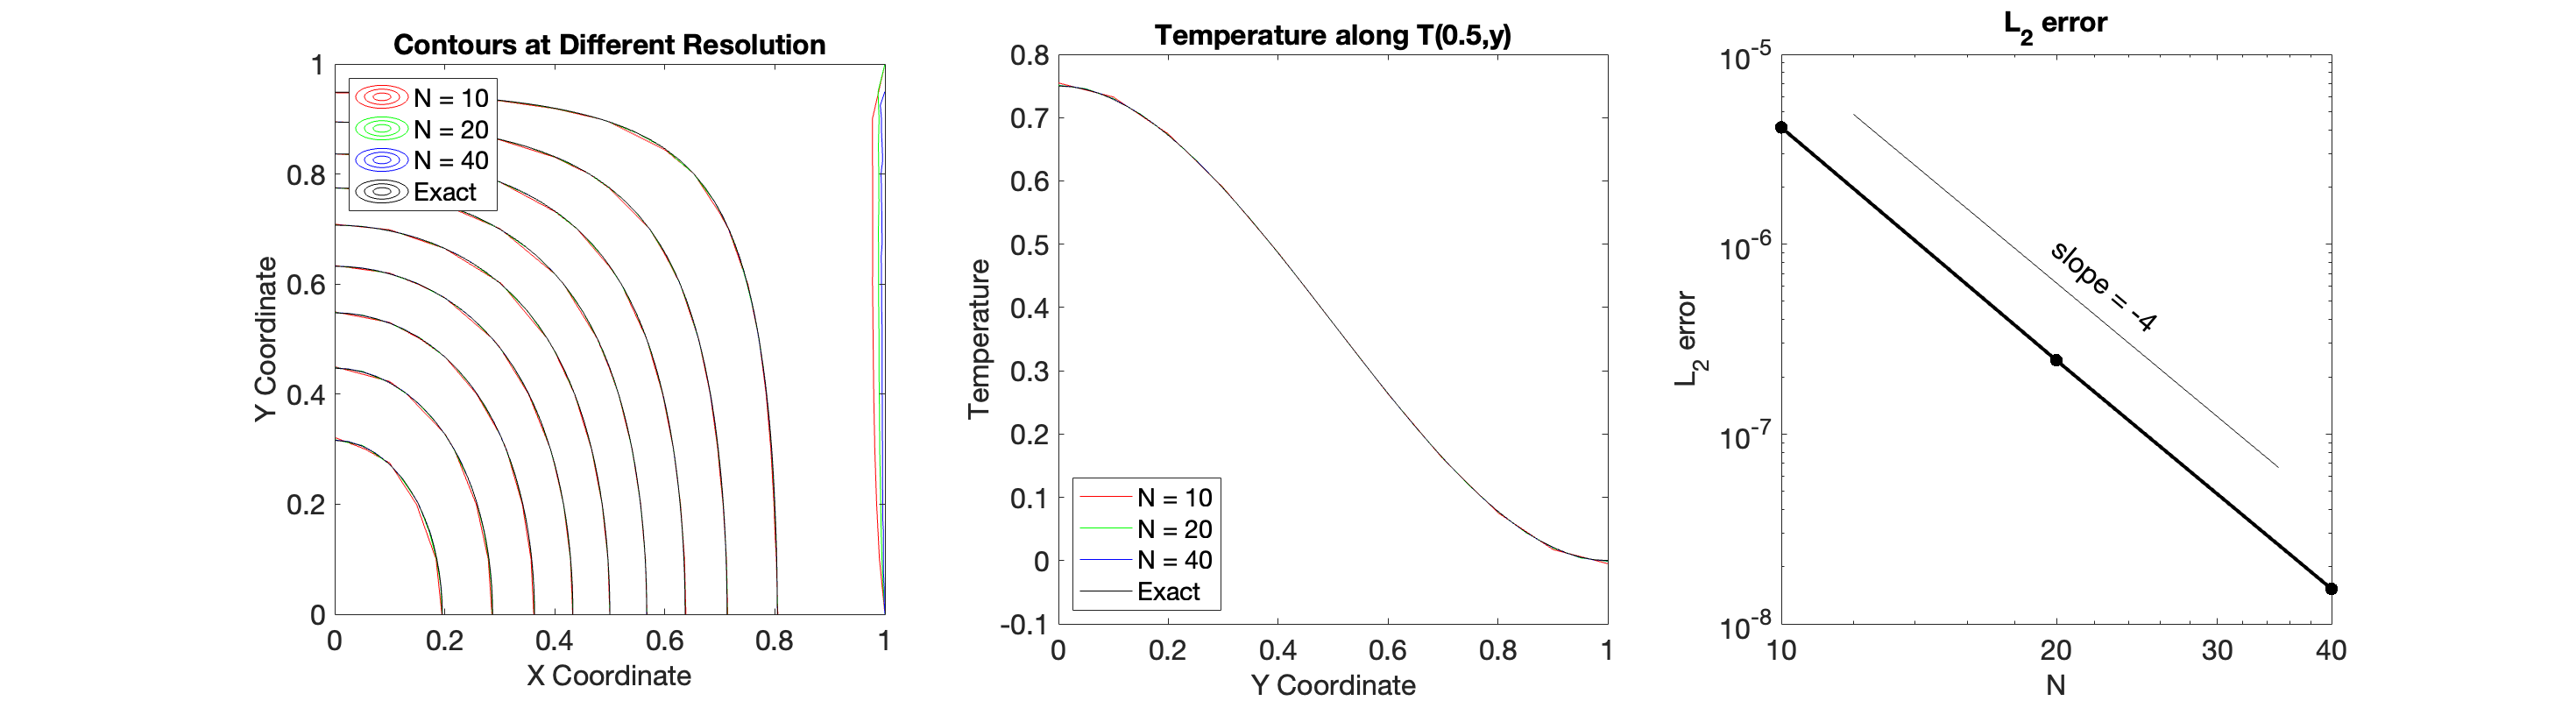
\includegraphics[width=\textwidth]{partC.png}
        \caption{Left: Contours of solution at different N.
            Center: Comparision of solution along T(y,0.5).
            right: Error as a function of N.}
            \label{fig:C}
    \end{figure}

    \section{Part D: Spatial Convergence of Gauss-Seidel}
    \noindent\Cref{fig:D} shows the spatial convergence using Gauss-Seidel iteration.
    At small resolutions, the method converges with fourth order accuracy.
    At higher resolutions, the convergence flatlines due to the first order approximations used for the no flux boundary conditions.
    \begin{figure}
        \centering
        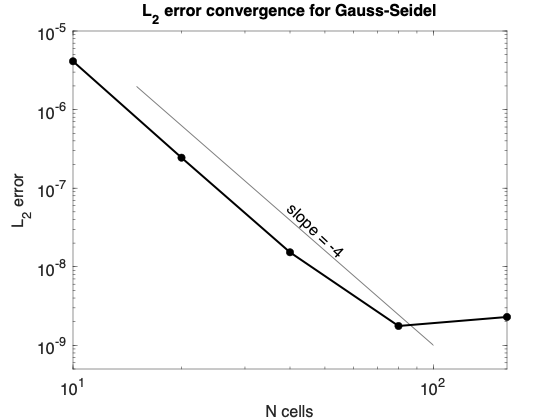
\includegraphics[width=0.33\textwidth]{partD.png}
        \caption{Error vs. N for the Gauss-Seidel iteration.}
        \label{fig:D}
    \end{figure}

    \section{Part E: Residuals as a function of iteration}
    \noindent \Cref{fig:E} shows the residual as a function of iteration count for Jacobi Iteration, Gauss-Seidel iteration, and Successive overrelaxtion at a variety of $\omega$'s.
    The convergence of SOR monotonically improves at $\omega$ ranges from $1.1$ to $1.9$.
    Above $\omega = 1.9$ however more iterations are required and the method eventually diverges.
    Jacobi iteration takes the longest to converge, followed by Gauss-Seidel while SOR converges the quickest as expected.
    \begin{figure}
        \centering
        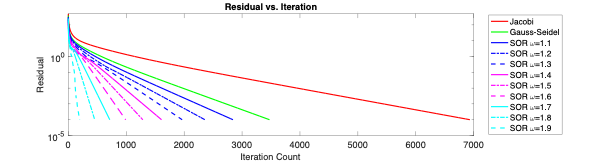
\includegraphics[width=\textwidth]{partE.png}
        \caption{Residual vs. iteration count for the implemented iterative schemes.}
        \label{fig:E}
    \end{figure}

    \section{Part F: Runtime}
    \noindent \Cref{fig:F} shows the runtime as a function of N for Jacobi iteration, Gauss-Seidel Iteration, and SOR.
    Red lines show the average time per iteration and blue lines show the time to convergence.
    The average time per iteration appears to have $\mathcal{O}(N^2)$ time complexity for all methods which is expected because the number of unknowns grows with $N^2$.
    Total run time appears to have $\mathcal{)}(N^4)$ time compleity, suggesting that the number of iterations required to reach convergence grows with $N^2$.
    This trend seems reasonable given that the number of unknowns grow with $N^2$ and information can only travel from each grid point and its neighbors at each iteration.
    \begin{figure}
        \centering
        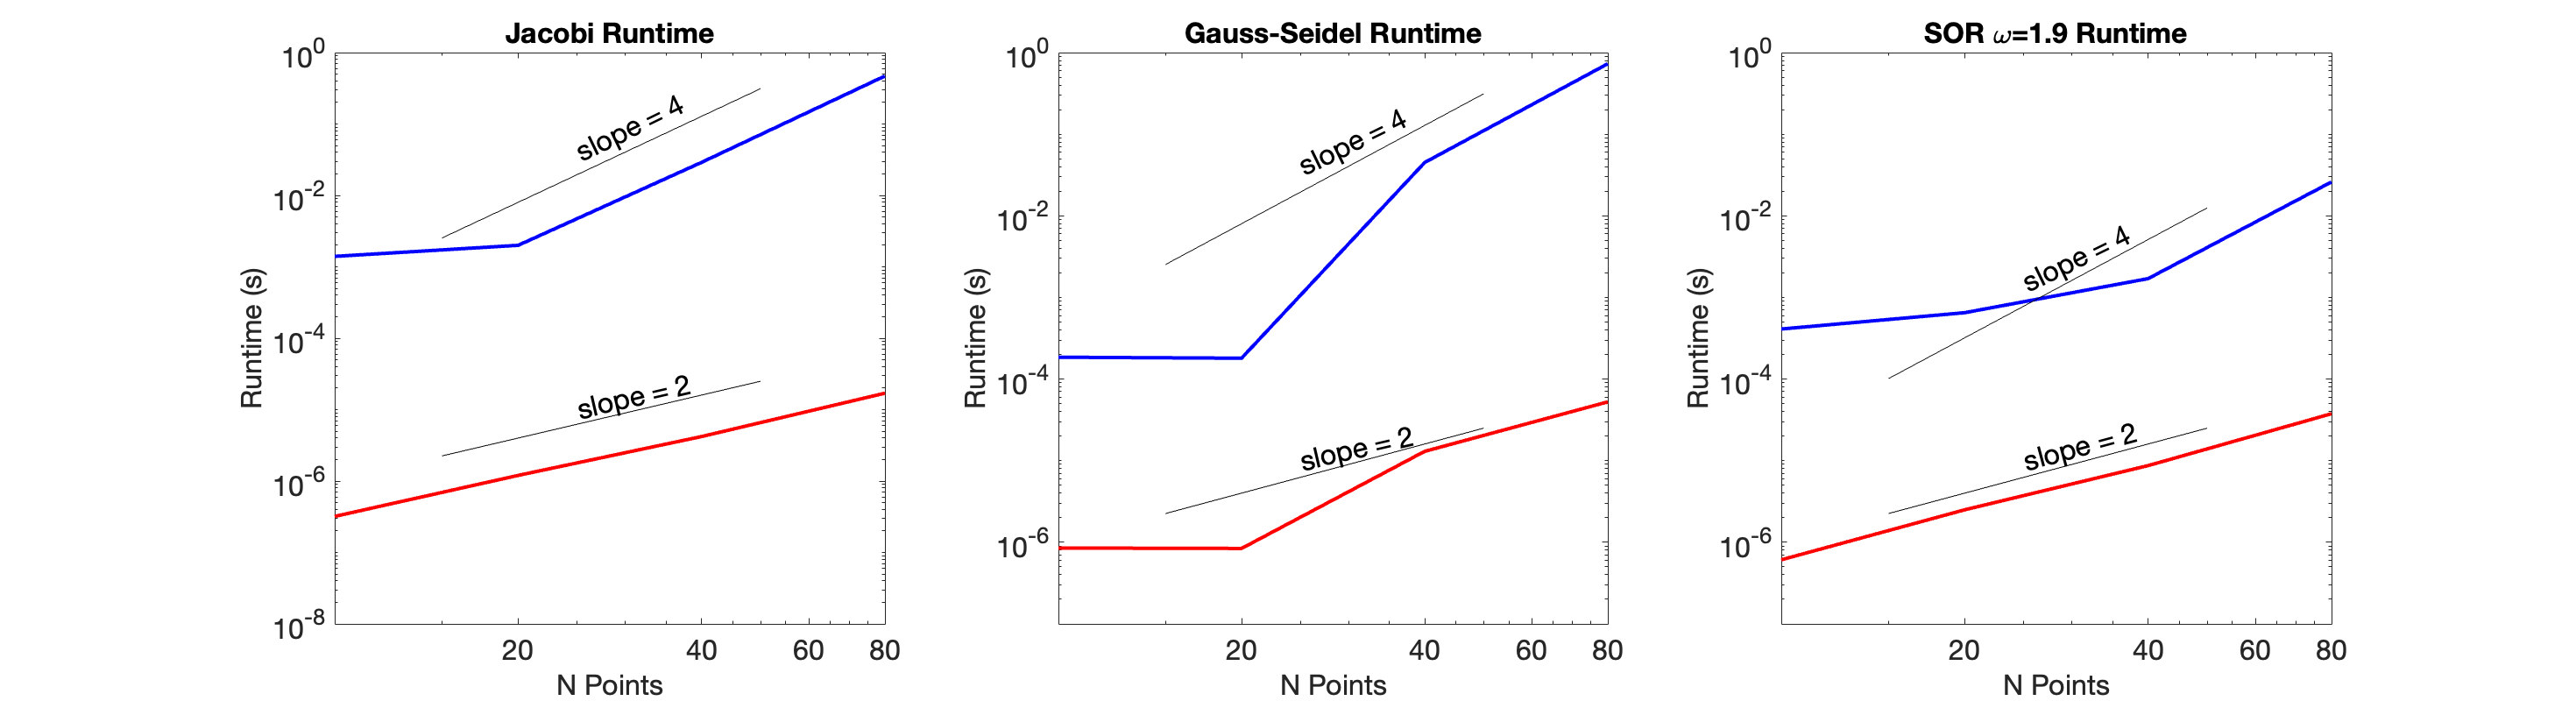
\includegraphics[width=\textwidth]{partF.png}
        \caption{Runtime as a function of N}
        \label{fig:F}
    \end{figure}

    \section{Part G: 2-Level Multigrid}
    \noindent\Cref{fig:G} shows the time to convergence for all four methods.
    The algebraic multigrid approach is two orders of magnitude faster than the simple single mesh iterative approaches.
    The implemente two level multigrid method performs five smoothing iterations on the fine mesh before solving for the error on the coarse mesh and applying the correction to the fine mesh.
    While Jacobi, Gauss-Seidel, and SOR all require hundreds to thousands of iterations with $N=$4, the algebraic multigrid converges in just six iterations comprising of 30 gauss-seidel iterations on the fine mesh.
    \begin{figure}
        \centering
        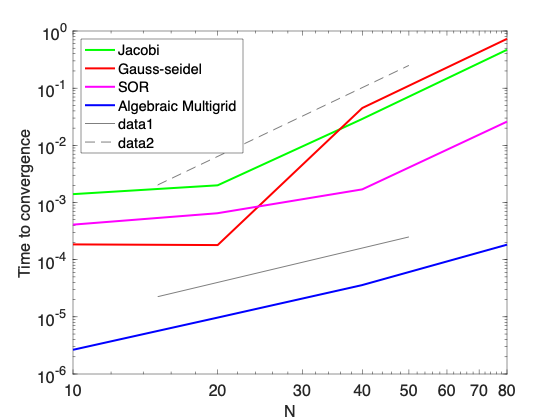
\includegraphics[width=0.33\textwidth]{partG.png}
        \caption{Time to convergence comparision of all methods}
        \label{fig:G}
    \end{figure}

\end{document}

